\documentclass[]{article}
\usepackage{lmodern}
\usepackage{amssymb,amsmath}
\usepackage{ifxetex,ifluatex}
\usepackage{fixltx2e} % provides \textsubscript
\ifnum 0\ifxetex 1\fi\ifluatex 1\fi=0 % if pdftex
  \usepackage[T1]{fontenc}
  \usepackage[utf8]{inputenc}
\else % if luatex or xelatex
  \ifxetex
    \usepackage{mathspec}
  \else
    \usepackage{fontspec}
  \fi
  \defaultfontfeatures{Ligatures=TeX,Scale=MatchLowercase}
\fi
% use upquote if available, for straight quotes in verbatim environments
\IfFileExists{upquote.sty}{\usepackage{upquote}}{}
% use microtype if available
\IfFileExists{microtype.sty}{%
\usepackage{microtype}
\UseMicrotypeSet[protrusion]{basicmath} % disable protrusion for tt fonts
}{}
\usepackage[margin=1in]{geometry}
\usepackage{hyperref}
\hypersetup{unicode=true,
            pdftitle={Supplementary Materials: A gene-diet interaction-based score predicts response to dietary fat in the Women's Health Initiative},
            pdfborder={0 0 0},
            breaklinks=true}
\urlstyle{same}  % don't use monospace font for urls
\usepackage{graphicx,grffile}
\makeatletter
\def\maxwidth{\ifdim\Gin@nat@width>\linewidth\linewidth\else\Gin@nat@width\fi}
\def\maxheight{\ifdim\Gin@nat@height>\textheight\textheight\else\Gin@nat@height\fi}
\makeatother
% Scale images if necessary, so that they will not overflow the page
% margins by default, and it is still possible to overwrite the defaults
% using explicit options in \includegraphics[width, height, ...]{}
\setkeys{Gin}{width=\maxwidth,height=\maxheight,keepaspectratio}
\IfFileExists{parskip.sty}{%
\usepackage{parskip}
}{% else
\setlength{\parindent}{0pt}
\setlength{\parskip}{6pt plus 2pt minus 1pt}
}
\setlength{\emergencystretch}{3em}  % prevent overfull lines
\providecommand{\tightlist}{%
  \setlength{\itemsep}{0pt}\setlength{\parskip}{0pt}}
\setcounter{secnumdepth}{0}
% Redefines (sub)paragraphs to behave more like sections
\ifx\paragraph\undefined\else
\let\oldparagraph\paragraph
\renewcommand{\paragraph}[1]{\oldparagraph{#1}\mbox{}}
\fi
\ifx\subparagraph\undefined\else
\let\oldsubparagraph\subparagraph
\renewcommand{\subparagraph}[1]{\oldsubparagraph{#1}\mbox{}}
\fi

%%% Use protect on footnotes to avoid problems with footnotes in titles
\let\rmarkdownfootnote\footnote%
\def\footnote{\protect\rmarkdownfootnote}

%%% Change title format to be more compact
\usepackage{titling}

% Create subtitle command for use in maketitle
\providecommand{\subtitle}[1]{
  \posttitle{
    \begin{center}\large#1\end{center}
    }
}

\setlength{\droptitle}{-2em}

%  \title{Supplementary Materials: A gene-diet interaction-based score predicts
%response to dietary fat in the Women's Health Initiative}
%    \pretitle{\vspace{\droptitle}\centering\huge}
%  \posttitle{\par}
%    \author{}
%    \preauthor{}\postauthor{}
%    \date{}
%    \predate{}\postdate{}
  
\usepackage{booktabs}
\usepackage{longtable}
\usepackage{array}
\usepackage{multirow}
\usepackage{wrapfig}
\usepackage{float}
\usepackage{colortbl}
\usepackage{pdflscape}
\usepackage{tabu}
\usepackage{threeparttable}
\usepackage{threeparttablex}
\usepackage[normalem]{ulem}
\usepackage{makecell}
\usepackage{xcolor}

\usepackage{float}

\usepackage[labelformat=empty]{caption}

\begin{document}
%\maketitle

A gene-diet interaction-based score predicts response to dietary fat in the Women's Health Initiative. Westerman et al.; Online Supplementary Material

\newcommand{\beginsupplement}{%
        \setcounter{table}{0}
        \renewcommand{\thetable}{\arabic{table}}%
        \setcounter{figure}{0}
        \renewcommand{\thefigure}{\arabic{figure}}%
     }
%
        \setcounter{table}{0}
        \renewcommand{\thetable}{\arabic{table}}%
        \setcounter{figure}{0}
        \renewcommand{\thefigure}{\arabic{figure}}%

\begin{ThreePartTable}
\begin{TableNotes}
\item Power calculations were undertaken using the Quanto tool, with parameters set as follows: additive model, SNP main effect of 0.5\% of trait variance, binary environment with 50\% prevalence, and environmental effect explaining 10\% of the trait variance.
\end{TableNotes}
\begin{longtable}[t]{rrrr}
\caption{\label{tab:show-power-calcs}Supplementary Table 1: Sample size necessary to achieve power of 0.8}\\
\toprule
GxE variance explained (\%) & N (nominal) & N (suggestive) & N (genome-wide)\\
\midrule
0.05 & 14046 & 49488 & 70866\\
0.10 & 7021 & 24737 & 35423\\
0.50 & 1401 & 4936 & 7069\\
1.00 & 699 & 2461 & 3524\\
\bottomrule
\insertTableNotes
\end{longtable}
\end{ThreePartTable}

\begin{ThreePartTable}
\begin{TableNotes}
\item[1] Sample size available with 1-year follow-up for each CRF
\item[2] Number of SNPs selected by the pruning-and-thresholding algorithm for each CRF-threshold combination
\item[3] Standardized effect size (SES) represents the regression coefficient estimate in terms of CRF standard deviation per responder score standard deviation
\end{TableNotes}
\begin{longtable}[t]{lllllllllll}
\caption{\label{tab:show-test-scores-alternate-filters}Supplementary Table 2: Responder score effects on CRF changes in DM trial participants across main-effect filter thresholds}\\
\toprule
\multicolumn{2}{c}{ } & \multicolumn{3}{c}{All variants} & \multicolumn{3}{c}{Nominal main effect (p<0.05)} & \multicolumn{3}{c}{Suggestive main effect (p<1e-5)} \\
\cmidrule(l{3pt}r{3pt}){3-5} \cmidrule(l{3pt}r{3pt}){6-8} \cmidrule(l{3pt}r{3pt}){9-11}
CRF & N\textsuperscript{1} & \# SNPs\textsuperscript{2} & SES\textsuperscript{3} & P-value & \# SNPs\textsuperscript{2} & SES\textsuperscript{3} & P-value & \# SNPs\textsuperscript{2} & SES\textsuperscript{3} & P-value\\
\midrule
BMI & 1988 & 158365 & 0.058 & 0.009 & 6042 & 0.029 & 0.189 & 569 & 0.027 & 0.221\\
SBP & 2004 & 153942 & -0.016 & 0.473 & 1536 & 0.034 & 0.125 & 6 & -0.003 & 0.899\\
LDL-C & 145 & 156313 & 0.124 & 0.337 & 1760 & -0.191 & 0.02 & 46 & 0.000 & 1.000\\
HDL-C & 150 & 153942 & 0.031 & 0.611 & 1731 & -0.083 & 0.32 & 42 & 0.086 & 0.244\\
TG & 150 & 152006 & -0.067 & 0.66 & 1774 & -0.146 & 0.055 & 47 & -0.034 & 0.661\\
FG & 281 & 161906 & -0.056 & 0.64 & 1924 & 0.011 & 0.853 & 7 & 0.004 & 0.952\\
\bottomrule
\insertTableNotes
\end{longtable}
\end{ThreePartTable}

\newpage

Online Supplementary Material: A gene-diet interaction-based score
predicts response to dietary fat in the Women's Health Initiative

\begin{ThreePartTable}
\begin{TableNotes}
\item[1] Sample size available with 1-year follow-up measurements for each CRF
\item[2] Std. effect size represents the regression coefficient estimate in terms of CRF standard deviation per responder score standard deviation
\end{TableNotes}
\begin{longtable}[t]{llllllllll}
\caption{\label{tab:show-test-scores-cross-ancestry}Supplementary Table 3: Responder score effects on CRF changes in DM trial participants across ancestries}\\
\toprule
\multicolumn{1}{c}{} & \multicolumn{3}{c}{All combined} & \multicolumn{3}{c}{Black} & \multicolumn{3}{c}{Hispanic} \\
\cmidrule(l{3pt}r{3pt}){2-4} \cmidrule(l{3pt}r{3pt}){5-7} \cmidrule(l{3pt}r{3pt}){8-10}
CRF & N\textsuperscript{1} & SES\textsuperscript{2} & P-value & N\textsuperscript{1} & SES\textsuperscript{2} & P-value & N\textsuperscript{1} & SES\textsuperscript{2} & P-value\\
\midrule
BMI & 3606 & -0.019 & 0.263 & 1214 & 0.002 & 0.941 & 404 & 0.019 & 0.714\\
SBP & 3645 & 0.046 & 0.005 & 1230 & 0.011 & 0.692 & 411 & -0.016 & 0.744\\
LDL-C & 422 & 0.084 & 0.068 & 206 & 0.06 & 0.373 & 71 & 0.124 & 0.24\\
HDL-C & 430 & -0.059 & 0.24 & 206 & -0.087 & 0.242 & 74 & -0.032 & 0.815\\
TG & 430 & -0.073 & 0.122 & 206 & -0.02 & 0.778 & 74 & -0.1 & 0.424\\
FG & 572 & 0.077 & 0.048 & 214 & -0.01 & 0.876 & 77 & 0.006 & 0.961\\
\bottomrule
\insertTableNotes
\end{longtable}
\end{ThreePartTable}

\begin{ThreePartTable}
\begin{TableNotes}
\item[1] Standardized effect size (SES) represents the regression coefficient estimate in terms of CRF standard deviation per responder score standard deviation
\end{TableNotes}
\begin{longtable}[t]{lllllll}
\caption{\label{tab:show-test-scores-ldpred}Supplementary Table 4: LDpred-based responder score effects on CRF changes in DM trial participants across causal variant fractions (F)}\\
\toprule
\multicolumn{1}{c}{ } & \multicolumn{2}{c}{F = 0.001} & \multicolumn{2}{c}{F = 0.01} & \multicolumn{2}{c}{F = 0.1} \\
\cmidrule(l{3pt}r{3pt}){2-3} \cmidrule(l{3pt}r{3pt}){4-5} \cmidrule(l{3pt}r{3pt}){6-7}
CRF & SES\textsuperscript{1} & P-value & SES\textsuperscript{1} & P-value & SES\textsuperscript{1} & P-value\\
\midrule
BMI & 0.001 & 0.969 & 0.003 & 0.906 & 0.003 & 0.906\\
SBP & -0.016 & 0.478 & -0.011 & 0.617 & -0.011 & 0.625\\
LDL-C & -0.038 & 0.652 & -0.051 & 0.555 & -0.053 & 0.533\\
HDL-C & 0.059 & 0.484 & 0.069 & 0.422 & 0.071 & 0.409\\
TG & 0.015 & 0.863 & 0.019 & 0.828 & 0.018 & 0.832\\
FG & 0.038 & 0.538 & 0.051 & 0.399 & 0.052 & 0.395\\
\bottomrule
\insertTableNotes
\end{longtable}
\end{ThreePartTable}

\begin{ThreePartTable}
\begin{TableNotes}
\item[1] Sample size available with 1-year follow-up measurements for each CRF
\item[2] Std. effect size represents the regression coefficient estimate in terms of CRF standard deviation per responder score standard deviation
\end{TableNotes}
\begin{longtable}[t]{lrrrr}
\caption{\label{tab:show-test-ldl-scores-other-rfs}Supplementary Table 5: LDL-FRS effects on alternate CRF changes in DM trial participants}\\
\toprule
Outcome risk factor & \# SNPs in risk score & N\textsuperscript{1} & Std. effect size\textsuperscript{2} & P-value\\
\midrule
BMI & 1760 & 1988 & -0.02 & 0.48\\
SBP & 1760 & 2004 & 0.00 & 0.85\\
HDL-C & 1760 & 150 & -0.07 & 0.40\\
TG & 1760 & 150 & 0.11 & 0.18\\
FG & 1760 & 281 & 0.01 & 0.93\\
\bottomrule
\insertTableNotes
\end{longtable}
\end{ThreePartTable}

\newpage
Online Supplementary Material: A gene-diet interaction-based score
predicts response to dietary fat in the Women's Health Initiative

\begin{figure}[H]
\centering
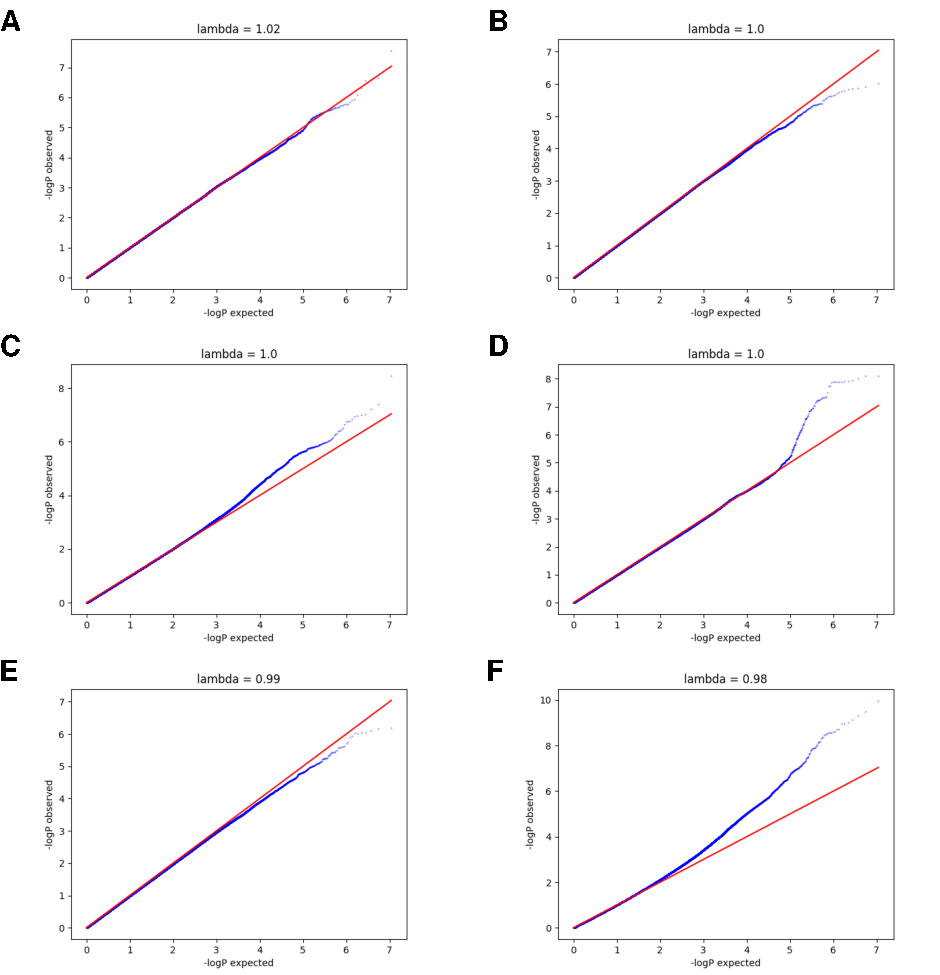
\includegraphics{figures/show-qq-plots-1.pdf}
\caption{Supplementary Figure 1: Q-Q plots from individual CRF GWIS. The distribution of
p-values from each GWIS is plotted against the expected uniform p-value
distribution. Plots correspond to: A) BMI, B) SBP, C) LDL-C, D) HDL-C,
E) TG, and F) FG. Lambda values above each plot represent genomic
inflation estimates. BMI: body mass index, SBP: systolic blood pressure,
LDL-C: LDL cholesterol, HDL-C: HDL cholesterol, TG: triglycerides, FG:
fasting glucose.}
\end{figure}


\end{document}
